
\Chapter{トーラスのタイヒミュラー空間\hspace{-.1em}I (浅香 猛)}


\Section{序}
形を知りたい―宇宙の形を知りたい、ある特定のタンパク質の形を知りたい―というような欲動はおそらく絶えずあって、調べ始めるにはどの範囲までの形を考えるのか、どの程度似ていたら同じものとみなすのか決めないといけない.ここで考えるのは、複素平面から作られるトーラス全体で、双正則同値になっているものは同じとみなす.さらにトーラスにマーキングをつけて、なお厳しい見方で、マーキングされたトーラスを類別する.このようなトーラス全体が、トーラスのタイヒミュラー空間である.この何を言ってるのか分からない話を分かるように、以下、努力していきたい.もし分からなかったら著者のせいである.

\Section{トーラス}
複素平面からトーラスを作る.複素平面とは、実数だけだと数が足りないために$1$乗して$-1$になる数$i$を加え、実数を拡張したものである.
\begin{wrapfigure}{r}{3cm} 
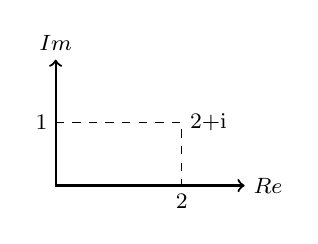
\begin{tikzpicture}[domain=-3:3, samples=64, scale=0.8]
\footnotesize
    \draw [<->,thick] (0,2) node (yaxis) [above] {$Im$}
        |- (3,0) node (xaxis) [right] {$Re$};
	\draw (2,1) coordinate (c);
	\coordinate [label=right:{2+i}] (2+i) at (2,1);
	\draw[dashed] (yaxis |- c) node[left] {$1$} -| (xaxis -| c) node[below] {$2$};

\end{tikzpicture}
\end{wrapfigure}
$(a+bi)+(c+di)=(a+c)+(b+d)i$\\
$(a+bi)(c+di)=(ac-bd)+(b+d)i$\\
($a$,$b$,$c$,$d$は実数)\\
と足し算、かけ算が定義され、引き算、割り算もそれから導かれる.
複素平面から何か平行四辺形を切り抜こう.例えば\\
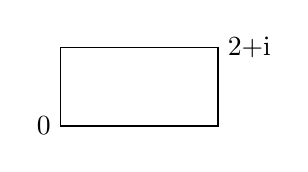
\begin{tikzpicture}
\draw (0,0) rectangle (2,1);
\coordinate [label=left:{0}] (0) at (0,0);
\coordinate [label=right:{2+i}] (2+i) at (2,1);
\end{tikzpicture}

を切り抜くことにする.そして、対辺をそれぞれ貼り合わせると
\begin{figure}[h]
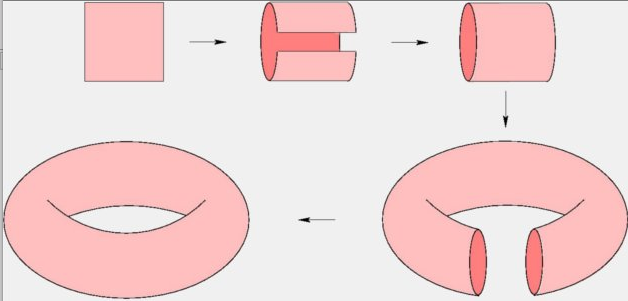
\includegraphics[width=5cm]{asaka3.png}
\end{figure}
とドーナツの表面となった.これがトーラスである.\\
実は切り抜くという操作はあまり良くない.なぜなら数学において境界は大事なのに、切り抜くと境界での構造がぐしゃぐしゃしてしまうからである.余裕のある人はもう少し良いイメージで考えてほしいのだが、それはトイレットペーパーである.切り抜いてしまわずに、複素平面全体をくるくると巻いていく.今回の例で行くと、0と2を結ぶ線分とiと2+iを結ぶ線分がぴたりと一致するように縦に巻き、以降同じ周期でくるくる巻くことにする.複素平面に厚さはないものと考えれば、このように巻ける.複素平面において0と2を結ぶ線分より下にある部分もすでに同じように巻かれていたとする.すると無限に重なった巻物が得られ、さらに0とiを結ぶ線分と2と2+iを結ぶ線分が重なるように横にも周期的に巻いていく.現実の紙だと紙が交差してできないが、この複素平面は自分を通り抜けられると考えれば巻いていける.これによって、平行四辺形が無限個重なったドーナツの表面がえられる.これがトーラスである.\\
複素平面から作り出したので、トーラスは、詳しくは説明できないが複素平面由来の構造を持っている。このトーラスは長方形の選び方によって形が違う気がする.この話を次の節にもっていく.

\Section{トーラスのモデュライ空間}
トーラスの形が同じであるということを双正則同値によって定める.双正則同値の説明は著者の力量不足のためうまくできない.それでも一応、大雑把に言うと、双正則同値とは、トーラスの持つ複素平面由来の構造が等しいということである.\\
また、別の言い方をしてみると、2つのトーラスA,Bに対して、双正則という性質を持つ変換によってAをBに変形できるとき、その2つは双正則であるという.これは、例えば、長方形に対して、相似という関係を、一方を拡大か縮小という変換を行ってもう一方に変形できることと説明するのと同じ言い方である.\\
双正則同値そのものは難しいが、トーラスをつくる型となった平行四辺形を用いると、双正則同値となる十分条件は説明できる.次の事実がある\\
「複素平面上に2つの平行四辺形A、Bがあったとする.Aを縦横比を保ったまま拡大か縮小をして、平行移動と回転移動をすることでBと重なるとき、AからつくられるトーラスとBからつくられるトーラスは双正則同値である」\\
たとえば\\ 
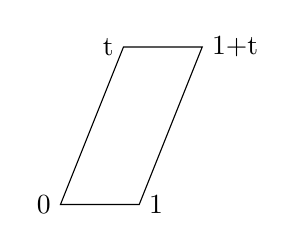
\begin{tikzpicture}
\coordinate [label=left:{0}] (A) at (0,0);
\coordinate [label=right:{1}](B) at (1,0);
\coordinate [label=left:{t}](C) at (0.8,2);
\coordinate [label=right:{1+t}](D) at (1.8,2);
\draw (A) -- (B) -- (D) -- (C) -- cycle;
\end{tikzpicture}

\begin{figure}[h]
\begin{minipage}{0.5\hsize}
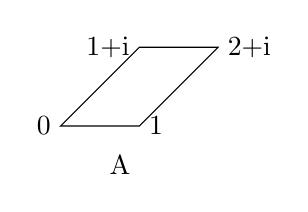
\begin{tikzpicture}
\coordinate [label=left:{0}] (A) at (0,0);
\coordinate [label=right:{1}](B) at (1,0);
\coordinate [label=left:{1+i}](C) at (1,1);
\coordinate [label=right:{2+i}](D) at (2,1);
\coordinate [label=right:{A}](E) at (0.5,-0.5);
\draw (A) -- (B) -- (D) -- (C) -- cycle;
\end{tikzpicture}
\end{minipage}
\begin{minipage}{0.5\hsize}
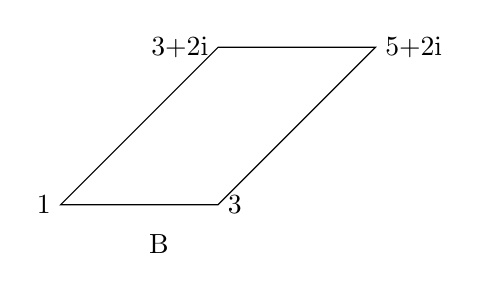
\begin{tikzpicture}
\coordinate [label=left:{1}] (A) at (0,0);
\coordinate [label=right:{3}](B) at (2,0);
\coordinate [label=left:{3+2i}](C) at (2,2);
\coordinate [label=right:{5+2i}](D) at (4,2);
\coordinate [label=right:{B}](E) at (1,-0.5);

\draw (A) -- (B) -- (D) -- (C) -- cycle;
\end{tikzpicture}
\end{minipage}
\end{figure}


のとき、AからつくられるトーラスとBからつくられるトーラスは同じものである.
このことから、tは複素平面上の実軸より上の領域(上半平面と名付ける)を自由に動くとして、以下の平行四辺形\\

図4.5\\

を考えれば、他のある位置にある平行四辺形からトーラスをつくったとしても、それに応じてtをうまく定めれば、 双正則同値なトーラスをつくれる.すなわち、tを動かして、0と1を結ぶ線分と0とtを結ぶ線分でできる平行四辺形全体を考えれば、すべてのトーラスは考えつくされる.\\
このことを踏まえ、さらに、次の、双正則同値と同値な条件がある.\\
「図5 と 図6 からつくられるトーラスが双正則同値$\Leftrightarrow $$s=\dfrac {at+b} {ct+d}$をみたす整数$a$、$b$、$c$、$d$が存在して、$ad-bc=1$となる」\\
だから例えば\\

図7\\

によってできるトーラスは双正則同値となる.この関係で互いに等しくならないt全体を挙げてみれば、分かったような気になる.これがトーラスのモデュライ空間呼ばれるもので\\

図8\\

これである.この斜線部上の点tをとり、そこから平行四辺形をつくれば、この型を元にトーラスがつくれる.\\

図9\\

つまり、この斜線部上の一点一点がトーラスに対応していて、トーラス全体というものを目の当たりにした.

\Section {トーラスのタイヒミュラー空間}
トーラス上に向きのある輪をおくと\\

図10\\

この2つの輪はトーラスから離れてしまわないようにどう伸び縮みさせても一点につぶせない.\\

図11\\

このような輪はトーラス上で縮めていけば一点につぶせる.\\
そのような一点につぶせない輪のかけ方はいくらでもある.ただし、トーラス上を移動して、重ねられるような輪のかけ方は同じとみなす.\\

図12\\

個の一点につぶせない輪のかけ方は、実は最初の2つを組み合わせてすべてつくれる.組み合わせるという言い方はあいまいだが、次の例でなんとなくわかって欲しい.\\

図13\\

実は最初の2つとは別のものからでもあらゆる輪のかけ方を作れる.たとえば\\

図14\\

でもよい.この輪のかけ方を生み出す元のものを”基本群の標準生成系”と呼ぶことにする.トーラスを一つ選び、さらにその”基本群の標準生成系”をひとつ選ぶことにする.このトーラスと”基本群の標準生成系”のペアを考える.トーラス全体はどのようなものか、前の章で見た.このトーラス一つ一つに標準生成系とのペアを考えることで種類を増やす.トーラスに標準生成系つけた印をマーキングと呼ぶ\\
もう一度tの動く範囲を上半平面として考える。上半平面上のそれぞれ別の場所にt、sがいても、前の章で言った条件「$s=\dfrac {at+b} {ct+d}$をみたす整数$a$、$b$、$c$、$d$が存在して、$ad-bc=1$となる」を満たせばそこからつくられるトーラスは双正則同値になるのだった.ここで0と1を結ぶ線分(直線でもよい)、1とtを結ぶ線分(直線でもよい)に注目すると、これらの線分(直線)はトーラス上で、”基本群の標準生成系”となっている.sのトーラスについても同じことを考えると”基本群の標準生成系”が得られる。この2つのトーラスは「$s=\dfrac {at+b} {ct+d}$をみたす整数$a$、$b$、$c$、$d$が存在して、$ad-bc=1$となる」を満たせば、双正則同値になるのだった.つまり、双正則な変換によってtのトーラスはsのトーラスに変形する.しかし”基本群の標準生成系”はどうかというと、証明は省くが、同じになる(tのトーラスをsのトーラスでうつす変換によってtの”基本群の標準生成系”をうつしたものが、トーラス上を動かすことでsの”基本群の標準生成系”に一致させられる)とは限らないのだ.今回は、双正則同値になるだけでなく”基本群の生成元”も含めて一致するものを同じとみなす厳しい見方を採用する.\\

図15\\

次の事実がある.\\
「図16と 図17からつくられるマーキングされたトーラスが同じになる$\Leftrightarrow $ $t=s$」\\
これにより、マーキングされたトーラス全体は上半平面と一致する.この上半平面の一点一点がそれぞれ異なるマーキングされたトーラスに対応する.そして、これがトーラスのタイヒミュラー空間である.

図17







